\section{Sistema Operativo}
    Para el presente proyecto se desarrollo un sistema operativo
    para el ESP-32, a este se le denomino como CodeGrav.

    \subsection{Caracteristicas}
        \begin{itemize}
            \item Booteo dinamico a diferentes programas, creando un ambiente preconfigurado.
            \item Modular lo que permite elasticidad en el diseño y la seleccion de sensores, ya que el kernel es generico.
            \item Manejo de Bluetooth de baja energia de forma paralela.
            \item Uso de System Calls como \acrshort{api} entre los programas y el kernel, al hacer eso de esa arquitectura, nuestro programa principal post kernel, no necesita saber nada sobre los sensores, o su tipo de dato, 
            ya que el kernel se encarga de esto.
        \end{itemize}
    
    \begin{figure}[htp!]
        \centering
        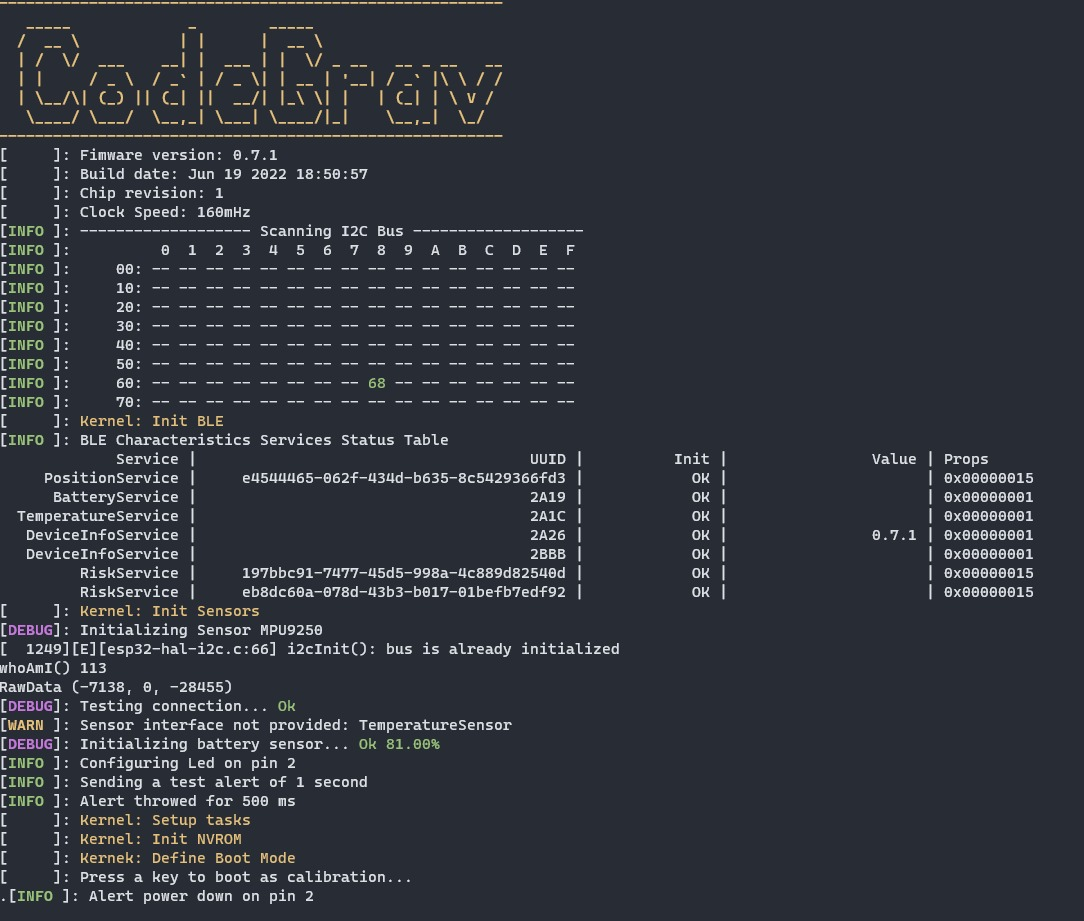
\includegraphics[width = 0.35 \textwidth]{SO.jpg}
        \caption{Secuencia de boot}
        \label{fig: boot_sequence}
    \end{figure}
    \FloatBarrier

    En la fig \ref{fig: boot_sequence} se muestra la sequencia de boot. Esta secuencia esta
    definida por el siguiente diagrama:

    \begin{figure}[htp!]
        \centering
        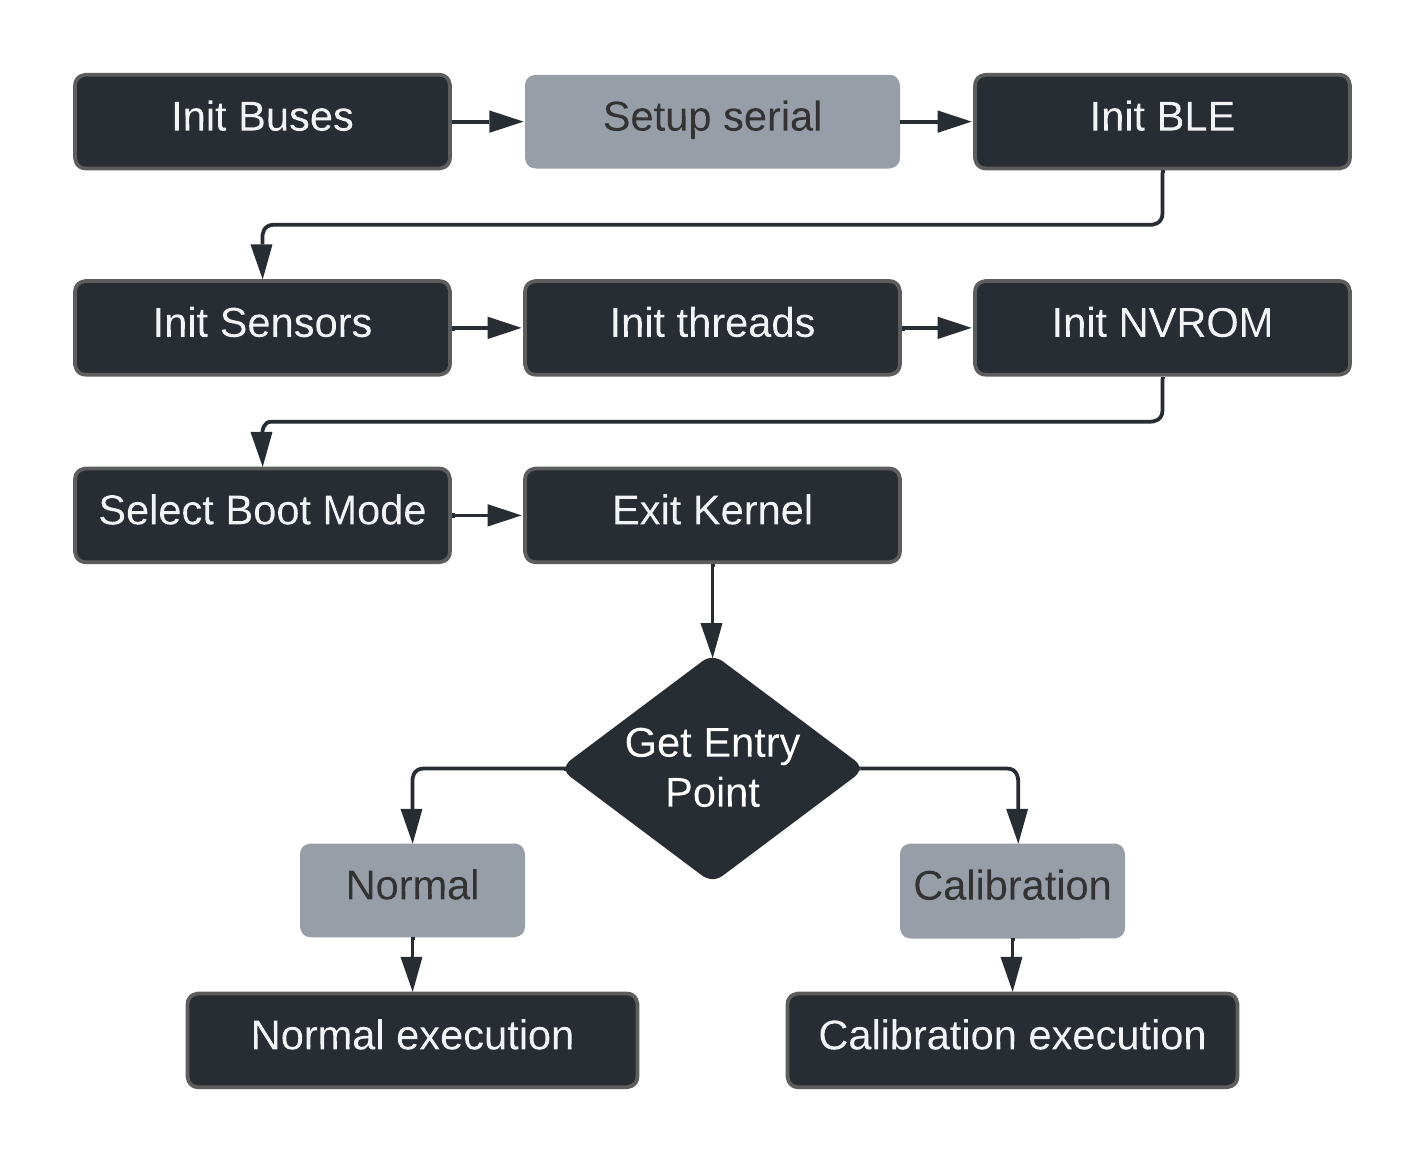
\includegraphics[width = 0.35 \textwidth]{boot_diagram_2.png}
        \caption{Diagrama de la secuencia de boot}
        \label{fig: boot_sequence_diagram}
    \end{figure}
    \FloatBarrier

    \begin{figure}[htp!]
        \centering
        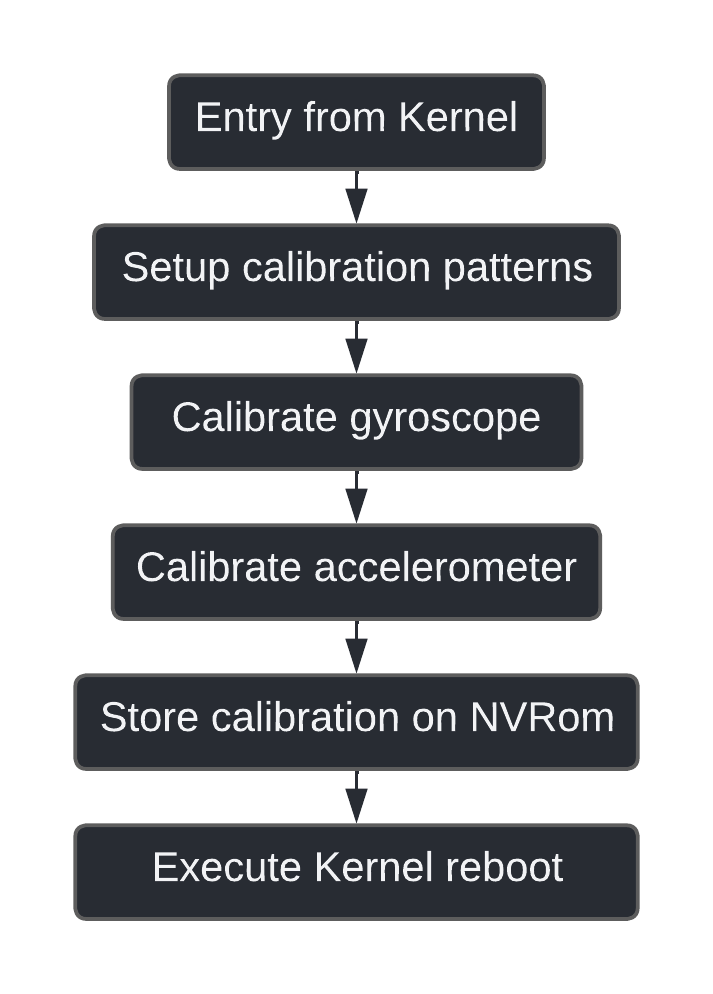
\includegraphics[width = 0.30 \textwidth]{calibration_execute.png}
        \caption{Diagrama de la secuencia de calibración.}
        \label{fig: calibration_diagram}
    \end{figure}
    \FloatBarrier

    \begin{figure}[htp!]
        \centering
        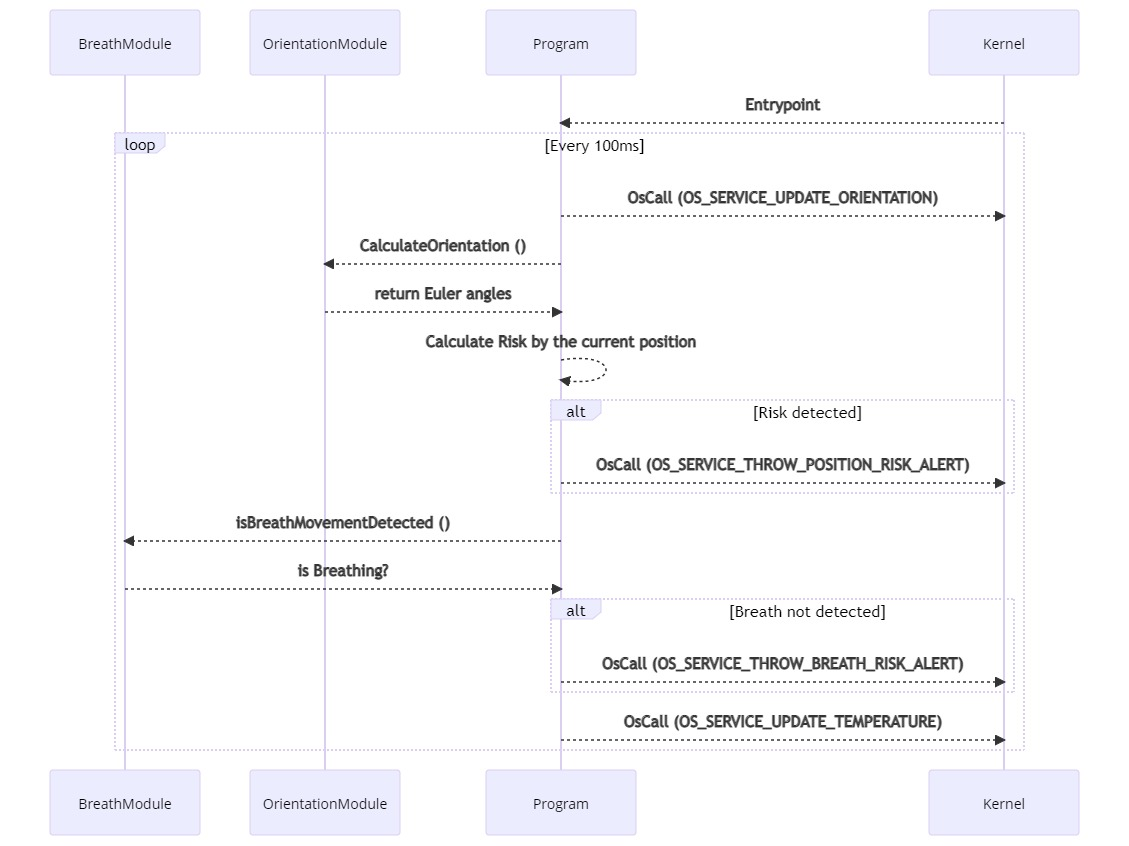
\includegraphics[width = 0.35 \textwidth]{normal_execute.jpg}
        \caption{Diagrama de la ejecución normal}
        \label{fig: normal_execution_diagram}
    \end{figure}
    \FloatBarrier


    

